\documentclass[11pt]{article}

\usepackage[utf8]{inputenc}
\usepackage[margin=2cm]{geometry}
\usepackage{cite}
\usepackage{natbib}
\usepackage{bibentry}
\usepackage{hyperref}
\usepackage{outlines}
\usepackage{enumitem}
\usepackage{graphicx}
%\setenumerate[1]{label=\Roman*.}
%\setenumerate[2]{label=\Alph*.}
%\setenumerate[3]{label=\roman*.}
%\setenumerate[4]{label=\alph*.}

\nobibliography*
	
\begin{document}
	
	\title{An Introduction to Egyptian Hieroglyphs -- CRN 11077}
	\author{C. Casey \\
		Wilbour Hall 302 \\
  		\texttt{\href{mailto:christian_casey@brown.edu}{christian\_casey@brown.edu}}}
	\date{\today}
	\maketitle
	
	\section*{Class Meeting Time/Place}
	
		\begin{tabular}{l l}
		Date: & July 17 – July 21, 2017 \\
		Time: & 15:30 – 18:20 \\
		Place: & TBD
		\end{tabular} 
		
% Description		
	\section*{List of Supplies}
		\begin{enumerate}
			\item White papyrus ($\approx$ 1 large sheet per 4 students)
			\item India ink ($\approx$ 1 jar per 4 students)
			\item Black acrylic paint (1)
			\item Acrylic matte medium (1)
			\item Dip pens (1 per student)
		\end{enumerate}
		
		The sheets of papyrus (as sold by the RISD Store) are large and can be cut into several pieces.
		The ink, paint, and medium will be combined to create an imitation of ancient Egyptian ink that looks realistic on papyrus but doesn't smudge.
		The dip pens are the closest analogue to an ancient Egyptian reed pen. 
		The cheapest available pens are perfectly suited to the needs of the activity.
		
		
		\begin{figure}[!h]
		\centering
		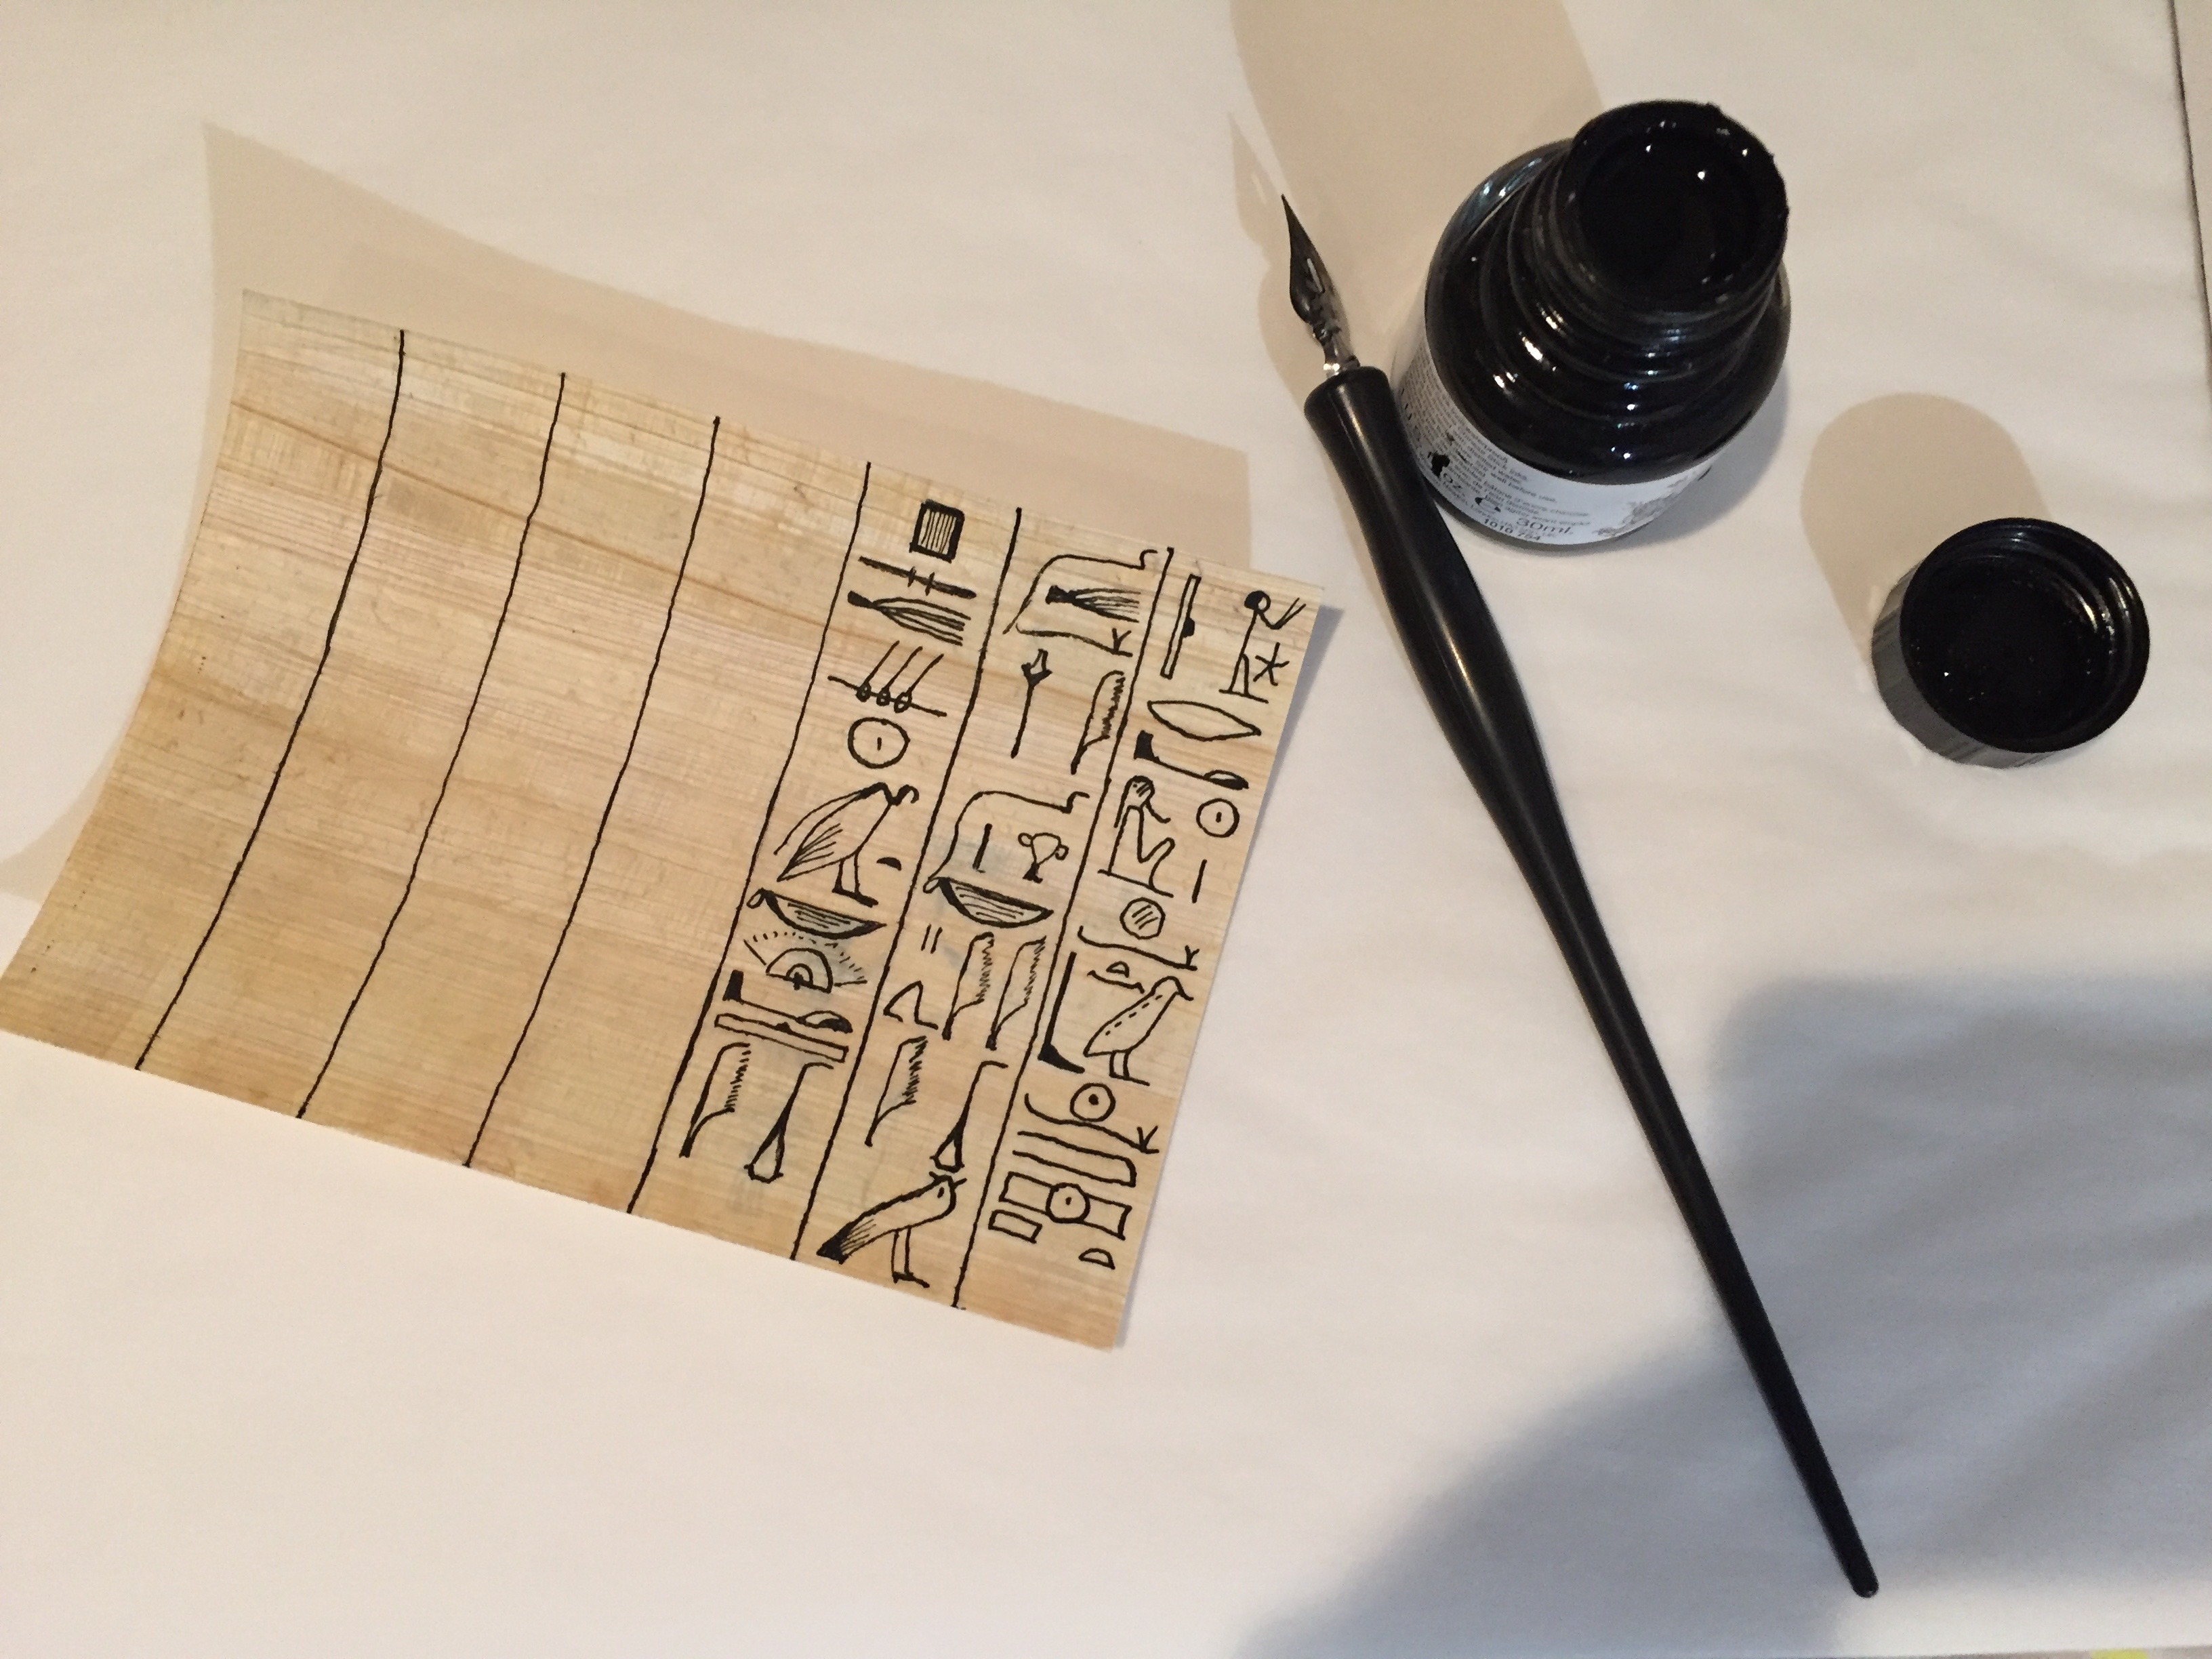
\includegraphics[width=0.5\textwidth]{cursive}
		\caption{Modern recreation of a cursive hieroglyphic text created using the materials listed.}
		\end{figure}
		

\end{document}













